\documentclass[conference,10pt]{IEEEtran}
\IEEEoverridecommandlockouts
\usepackage[T1]{fontenc}
\usepackage{graphicx,booktabs,amsmath,amssymb,xcolor,url,xspace,textcomp}
\usepackage[hidelinks]{hyperref}
\hypersetup{pdftitle={Egocentric Human Demonstrations for Bimanual Garment Manipulation}, pdfauthor={Jeong Hwan Lee}}
\usepackage{array,tikz}
\usetikzlibrary{positioning,arrows.meta}
\newcommand{\mm}{\,mm\xspace}
\def\UrlBreaks{\do\/\do\_\do\.\do\-}\def\UrlFont{\small\ttfamily}\newcommand{\code}[1]{\path{#1}}
\DeclareMathOperator*{\argmin}{arg\,min}
\definecolor{humF}{HTML}{E3F2FD}\definecolor{humS}{HTML}{1E88E5}
\definecolor{trjF}{HTML}{E8F5E9}\definecolor{trjS}{HTML}{43A047}
\definecolor{robF}{HTML}{FFEBEE}\definecolor{robS}{HTML}{E53935}
\definecolor{calF}{HTML}{FFFDE7}\definecolor{calS}{HTML}{F9A825}
\definecolor{senF}{HTML}{ECEFF1}\definecolor{senS}{HTML}{546E7A}
\definecolor{polF}{HTML}{F3E5F5}\definecolor{polS}{HTML}{8E24AA}

\begin{document}
\title{Egocentric Human Demonstrations for\\Bimanual Garment Manipulation:\\[1mm]\Large From Hand-Worn-Gripper Recordings to Robot Policies}
\author{\IEEEauthorblockN{Jeong Hwan Lee}
\IEEEauthorblockA{Technical report, status of 5 November 2026\\
Repository: \texttt{egocentric-garment-manipulation}}}
\maketitle

\begin{abstract}
We want a two-arm robot to manipulate a T-shirt using human demonstrations recorded with hand-worn grippers, without
teleoperation and without robot data collection. The demonstrator wears two HandUMI grippers (an open-source design by
BrikHMP18, not ours) with fiducial markers, a wrist fisheye camera, an IMU and, since 29 October 2026, the jaw servo read
as a torque-off encoder; a fixed RGB-D camera observes both hands. All poses are expressed in one world frame, the robot
base, set by a camera-to-robot calibration (0.98\,px held-out), start markers measured in that frame and a calibrated
marker rig (1--4\mm static error), and all streams share one host clock. The jaw-tip pose comes from point tracking on the
fixed camera (CoTracker3) anchored by the markers, with the IMU only inside tracking gaps: on held-out takes the error at
hidden markers has a median of 16\mm (left) and 19\mm (right), against about 42\mm for markers with IMU fill alone;
wrist-camera SLAM was tried and rejected because it loses tracking exactly at grasps. As an end-to-end test of the data,
converted demonstrations were first replayed open loop on two reBot B601-DM arms: four replays of one 33\,s
demonstration repeat within about 1\mm, the jaws close 5--19\mm above the table (human about 10\mm), and the robot
grasped and dragged the shirt, but did not fold it. We then built policy training data: 300 successful T-shirt
flattening demonstrations, graded per demo, with labels taken \emph{before} inverse kinematics and without any clamp.
First fine-tuned policies, observed in robot trials that were not counted, stop short of the cloth and close the jaws
early. Two causes were recorded (the policy copied the jaw state from its input; the robot wrist cameras sit differently
from the hand-worn ones), and checking the labels found three more data problems (a label clamp, demonstration speed,
video jaw labels). In a reduced feasibility test, pinching one sleeve with the left hand, a policy fine-tuned on 197
demonstrations grasped the sleeve in real-robot trials on 2 November 2026; the trials were not counted, and after a miss
the policy grasps elsewhere instead of retrying. Back on flattening, a policy trained with the cloth-folding recipe of
UMI on 250 demonstrations under a re-aimed camera improves its offline score from epoch to epoch, and a vision
classifier now labels whether a closed jaw holds the cloth, because the jaw servo has no load signal. We report no
success rate.
\end{abstract}

% =====================================================================
\section{Introduction}\label{sec:intro}
Folding a T-shirt is long-horizon, bimanual and contact-rich, and the cloth state changes with every grasp. Teleoperated
robot data for such tasks is slow and expensive to collect. Hand-held and hand-worn grippers in the style of
UMI~\cite{chi2024umi} let a person demonstrate with an end-effector that resembles the robot's, without a robot in the
loop, so data collection scales with people rather than robots. The difficulty moves into the conversion: every error in
calibration, pose recovery, jaw labelling, timing or kinematic feasibility ends up in the training labels, and a policy
trained on those labels inherits it. Policy success rates are a late and indirect signal for such errors.

\textbf{Main question.} \emph{If a robot simply replays the converted human motion, open loop, does it do what the human
did?} Replay exercises every stage at once (calibration, pose, jaw state, robotization, IK, timing, control), puts human,
robot command and measured robot motion on one clock and in one frame so that errors can be attributed to a stage, and
fails visibly. The follow-up question is whether the same conversion yields labels from which a policy can learn a grasp.

\textbf{Contributions} of the work so far:
\begin{itemize}
\item one world frame, the robot base, set once by calibration and start markers, so that human and robot paths share it
  without per-take alignment (Sec.~\ref{sec:cal});
\item a pose source for hand-worn grippers that survives the grasp: fixed-camera point tracking anchored by fiducial
  markers, with the IMU only in gaps, validated at held-out markers (Sec.~\ref{sec:pose}); jaw labels from a servo
  encoder (Sec.~\ref{sec:jaw});
\item an open-loop replay test in which human, command and robot are compared on one clock, with its measured results
  (Sec.~\ref{sec:replay});
\item a training-data pipeline with per-demo grades and Cartesian labels before IK, the first policies on the robot, the
  recorded causes of their failure and the data problems found afterwards (Secs.~\ref{sec:data}--\ref{sec:policy}).
\end{itemize}

\textbf{Status} (2 November 2026). Replay is finished; folding by replay does not succeed. Policies fine-tuned on the
flattening data were run on the robot in uncounted trials and did not grasp. In a one-sleeve pinching test
(Sec.~\ref{sec:pinch}), successful grasps were observed in real-robot trials on 2 November; the trials were not
counted. No success rate is reported anywhere in this report, because no counted
trials were run.

\textbf{Relation to earlier versions.} This report replaces version 0.1 (27 October) and version 0 (21 October), which
described the replay track in full detail, and the short technical note; they are kept in \code{report/archive/}.
Replay-era details that no longer affect the current pipeline were removed here; superseded methods are summarised in
Table~\ref{tab:superseded}.

\begin{figure}[!t]
\centering
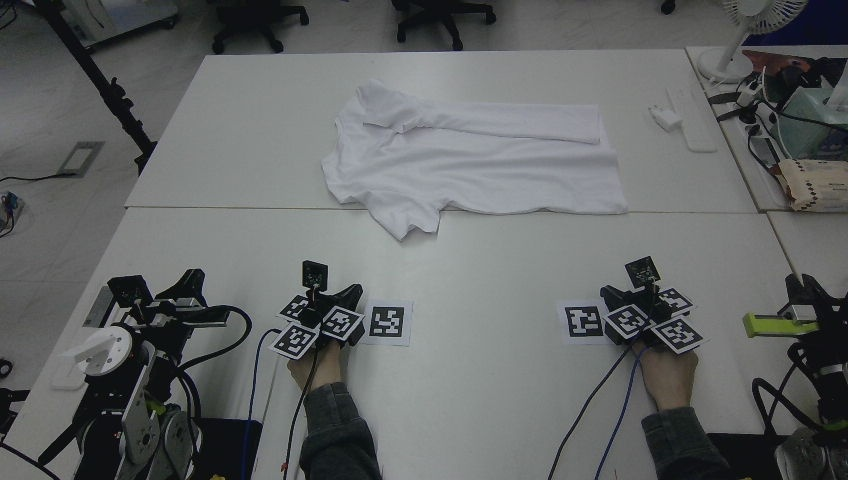
\includegraphics[width=\columnwidth]{figures/fig_scene.jpg}
\caption{The setup seen by the fixed RGB-D camera: a T-shirt on the table, the demonstrator's two hand-worn grippers
with fiducial markers resting on the two start markers, and the two robot arms at the left and right edges.}
\label{fig:scene}
\end{figure}

% =====================================================================
\section{Related Work}\label{sec:related}
\textbf{Hand-held and hand-worn grippers.} UMI~\cite{chi2024umi} records demonstrations with a hand-held parallel-jaw
gripper and a wrist fisheye camera; its pose comes from monocular-inertial SLAM based on
ORB-SLAM3~\cite{campos2021orbslam3}, and trajectories are filtered by the kinematics of the target robot.
HandUMI~\cite{handumi,meza2026handumi}, designed and published by BrikHMP18 and co-authors, is an open-source hand-worn
variant for robot-free bimanual data capture; we use a build copy of it. DexUMI~\cite{xu2025dexumi} uses the human hand
with an exoskeleton as the interface for dexterous hands. We keep the UMI-style gripper but take the pose from a fixed
RGB-D camera instead of wrist SLAM, and we test the data on the target robot before policy training. Instead of
removing infeasible trajectories, we keep the human path as the label and leave feasibility to the executor.

\textbf{Human data and low-cost bimanual robots.} EgoMimic~\cite{kareer2025egomimic} co-trains on egocentric human video
and robot data. ALOHA~\cite{zhao2023aloha} showed fine-grained bimanual manipulation with low-cost arms and teleoperation;
we use two low-cost reBot B601-DM arms but record without teleoperation, through LeRobot~\cite{cadene2024lerobot}.

\textbf{Cloth.} Garment folding and unfolding have been learned with dedicated primitives, e.g.\
SpeedFolding~\cite{avigal2022speedfolding} and FlingBot~\cite{ha2021flingbot}. We do not propose a cloth method; our
policies are generic diffusion-transformer~\cite{peebles2023dit} and VLA~\cite{xvla} policies.

\textbf{Pose, calibration, kinematics.} Markers are AprilTags~\cite{olson2011apriltag,wang2016apriltag2} detected with
OpenCV~\cite{bradski2000opencv}, solved with IPPE~\cite{collins2014ippe} and SQPnP~\cite{terzakis2020sqpnp}. Point tracking
uses CoTracker3~\cite{karaev2024cotracker3}; rotation uses a Mahony filter~\cite{mahony2008ahrs}. The camera-to-robot
solve is initialised with the method of Shah~\cite{shah2013robotworld}. IK uses Pink~\cite{pink} on
Pinocchio~\cite{carpentier2019pinocchio}. Evaluated and rejected as pose sources: MASt3R-SLAM~\cite{murai2025mast3rslam},
ORB-SLAM3, and with an earlier stereo camera Basalt~\cite{usenko2020basalt}, OpenVINS~\cite{geneva2020openvins} and
AirSLAM~\cite{xu2025airslam}.

% =====================================================================
\section{System Overview}\label{sec:overview}
\begin{figure*}[!t]
\centering
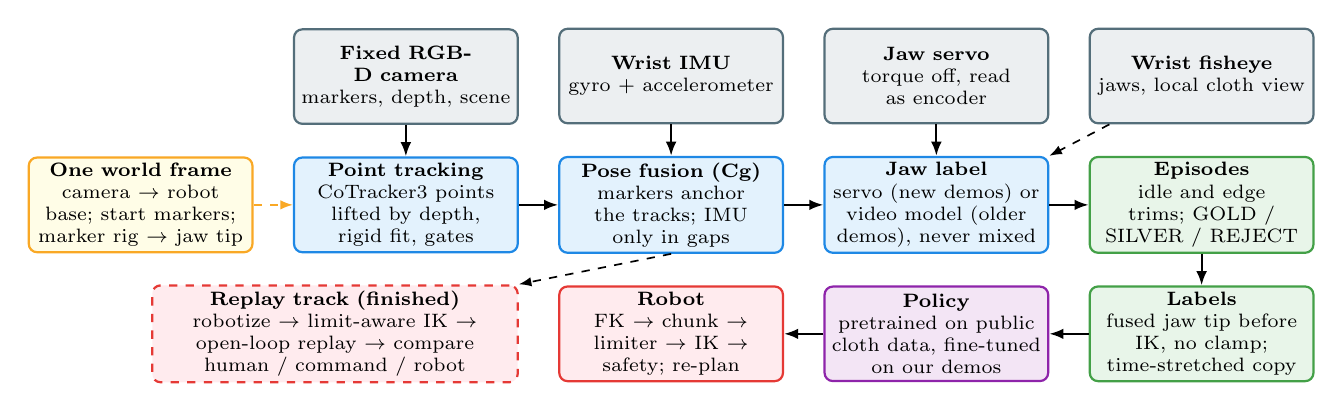
\begin{tikzpicture}[font=\scriptsize, node distance=4mm and 5mm,
  arr/.style={-{Latex[length=1.8mm]},thick},
  darr/.style={-{Latex[length=1.6mm]},dashed,semithick},
  box/.style={draw=#1S, fill=#1F, rounded corners=3pt, line width=0.8pt, text width=27mm, minimum height=12mm,
    align=center, inner sep=2pt}]
\node[box=cal] (cal) {\textbf{One world frame}\\camera $\to$ robot base; start markers; marker rig $\to$ jaw tip};
\node[box=hum, right=of cal] (pt) {\textbf{Point tracking}\\CoTracker3 points lifted by depth, rigid fit, gates};
\node[box=hum, right=of pt] (fu) {\textbf{Pose fusion (Cg)}\\markers anchor the tracks; IMU only in gaps};
\node[box=hum, right=of fu] (jw) {\textbf{Jaw label}\\servo (new demos) or video model (older demos), never mixed};
\node[box=trj, right=of jw] (gr) {\textbf{Episodes}\\idle and edge trims; GOLD / SILVER / REJECT};
\node[box=sen, above=of pt] (orb) {\textbf{Fixed RGB-D camera}\\markers, depth, scene};
\node[box=sen, above=of fu] (imu) {\textbf{Wrist IMU}\\gyro + accelerometer};
\node[box=sen, above=of jw] (srv) {\textbf{Jaw servo}\\torque off, read as encoder};
\node[box=sen, above=of gr] (fis) {\textbf{Wrist fisheye}\\jaws, local cloth view};
\node[box=trj, below=of gr] (lb) {\textbf{Labels}\\fused jaw tip before IK, no clamp; time-stretched copy};
\node[box=pol, left=of lb] (po) {\textbf{Policy}\\pretrained on public cloth data, fine-tuned on our demos};
\node[box=rob, left=of po] (dp) {\textbf{Robot}\\FK $\to$ chunk $\to$ limiter $\to$ IK $\to$ safety; re-plan};
\node[box=rob, dashed, left=of dp, text width=45mm] (rp) {\textbf{Replay track (finished)}\\robotize $\to$ limit-aware IK $\to$ open-loop replay $\to$ compare human / command / robot};
\draw[arr] (orb) -- (pt); \draw[arr] (pt) -- (fu); \draw[arr] (imu) -- (fu);
\draw[arr] (srv) -- (jw); \draw[darr] (fis) -- (jw.north east);
\draw[darr,draw=calS] (cal) -- (pt);
\draw[arr] (fu) -- (jw); \draw[arr] (jw) -- (gr); \draw[arr] (gr) -- (lb); \draw[arr] (lb) -- (po);
\draw[arr] (po) -- (dp); \draw[darr] (fu.south) -- (rp.north east);
\end{tikzpicture}
\caption{Data flow as of 1 November 2026. Grey: sensors, all stamped by one host clock. Yellow: one-time setup that
puts human and robot in one world frame. Blue: pose and jaw state of each gripper. Green: graded episodes and training
labels. Purple and red: policy and execution on the robot. Dashed box: the open-loop replay track, which tested the
conversion before policy training (Sec.~\ref{sec:replay}). The wrist video is a policy input; it supplies jaw labels only
for demonstrations recorded before the servo was reinstalled.}
\label{fig:pipe}
\end{figure*}

Figure~\ref{fig:pipe} shows the current data flow. Two principles run through it. \emph{One world frame}: every pose,
human or robot, is expressed in the robot base frame; no per-recording alignment (no SLAM map, no point-cloud
registration) is needed. \emph{One clock}: camera frames, IMU and servo samples and the robot's commanded and measured
joints all carry host timestamps, so human, command and robot can be compared sample by sample and filmed side by side
by the same camera without synchronisation hardware.

% =====================================================================
\section{Hardware}\label{sec:hw}
\begin{table}[t]
\caption{Components}\label{tab:hw}
\centering\small
\begin{tabular}{@{}>{\raggedright\arraybackslash}p{0.27\columnwidth}>{\raggedright\arraybackslash}p{0.65\columnwidth}@{}}
\toprule
unit & model, role \\
\midrule
Hand-worn gripper $\times$2 & HandUMI~\cite{handumi} by BrikHMP18 (not our design), our build; demonstration tool \\
Markers & three 48\mm AprilTags per gripper, since 23 October a fourth 30\mm tag on the back of the wrist camera \\
Wrist camera $\times$2 & fisheye, 1280$\times$720 at 30\,Hz; jaws and local cloth view \\
Wrist IMU $\times$2 & Seeed XIAO nRF52840 Sense; gyro and accelerometer \\
Jaw servo $\times$2 & Feetech STS3215, torque off, read at about 100\,Hz on the host clock (removed 13--28 October, back since 29 October) \\
RGB-D camera & Orbbec Gemini 336, colour + aligned depth (recorded at about 15\,Hz), fixed above the table; raised to 113\,cm on 25 October (height not re-measured after the angle-only re-aim of 1 November) \\
Robot arms $\times$2 & reBot B601-DM, 6-DoF + parallel jaw, Damiao motors on USB-CAN, our MIT-mode bridge at 100\,Hz \\
Host & Apple-silicon laptop: recording, IK, bridge, deploy loop \\
GPU & rented RTX 5090 pods for point tracking, the jaw model, the 3-D solve and some policy training; one run on a rented H100; RTX 4090 via Ray for the DiT fine-tunes \\
\bottomrule
\end{tabular}
\end{table}

\begin{figure}[!t]
\centering
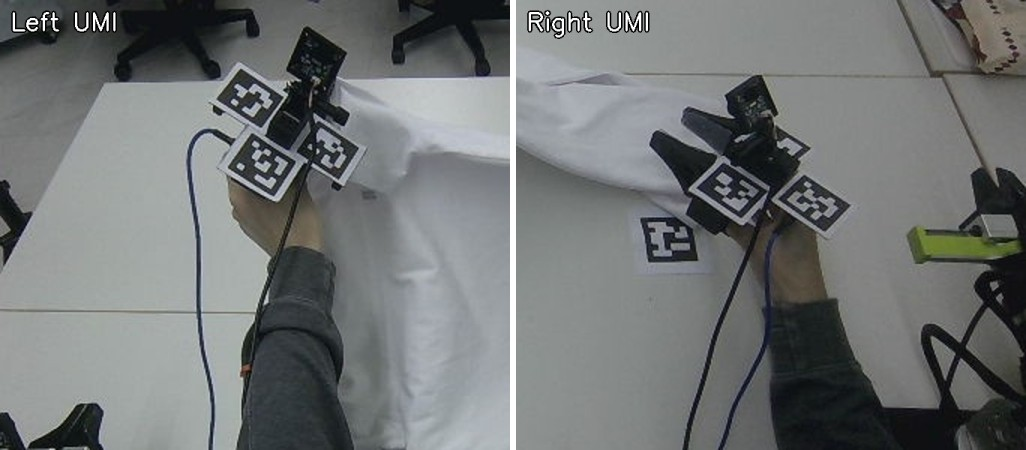
\includegraphics[width=\columnwidth]{figures/fig_umi.jpg}
\caption{The two hand-worn grippers as recorded before 23 October: HandUMI (BrikHMP18's design) with three 48\mm
AprilTags per hand, wrist fisheye and IMU; no jaw servo in that period. Since 23 October a fourth, 30\mm tag sits on the
back of each wrist camera, and since 29 October the jaw servo is back as an encoder.}
\label{fig:umi}
\end{figure}

Table~\ref{tab:hw} lists the components.

\textbf{HandUMI is not our design.} It was designed and published by BrikHMP18 (murobotics-ai,
\url{https://github.com/murobotics-ai/handumi-hw}, Apache-2.0)~\cite{handumi,meza2026handumi} and follows
UMI~\cite{chi2024umi}. We print the upstream parts (commit \texttt{e58de33}) and made these changes (Fig.~\ref{fig:umi}):
a wrist IMU instead of VR tracking; a modified controller-support connector, camera mount and servo cover; several
AprilTags per hand on different faces, so that at least one tends to face the fixed camera, plus since 23 October a small
tag on the back of the wrist camera, whose single-tag planar pose flip is resolved with the IMU.

\textbf{Jaw servo timeline.} The jaw servos were removed on 13 October, because the servo shafts broke and the units were
heavy; from 13 to 28 October the jaw state was inferred from the wrist video. On 29 October the servo was put back, now
with torque off so that it never drives the jaw while a person holds it; it is only read, as an encoder of the jaw
opening (Sec.~\ref{sec:jaw}).

\textbf{Robot.} Two reBot B601-DM arms (the vendor LeRobot plugin and URDF are not included in the repository) are driven
by our HTTP bridge in MIT mode: one 100\,Hz thread, acceleration-limited motion toward each goal, goal interpolation
between streamed commands, automatic re-enable of a disabled motor, USB reconnect, and an enforced jaw-opening limit.
The bridge uses an integral-only feed-forward torque and no gravity model; Sec.~\ref{sec:replay} explains why this
determined the tracking error.

% =====================================================================
\section{One World Frame and Calibration}\label{sec:cal}
\begin{figure*}[!t]
\centering
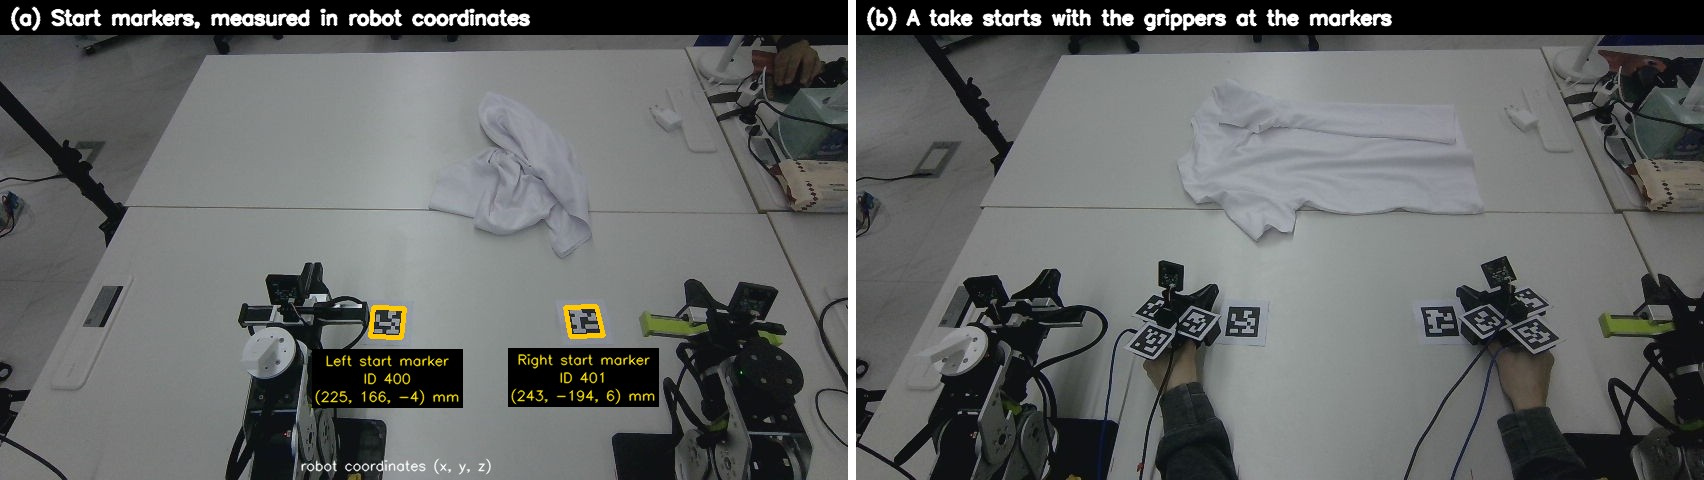
\includegraphics[width=0.85\textwidth]{figures/fig_start_markers.jpg}
\caption{Start markers. (a) Two AprilTags taped on the table (IDs 400 left, 401 right), measured once with the
calibrated fixed camera; their centres in robot coordinates are shown. (b) Every take starts with the two grippers at
these markers, so each demonstration begins at known robot coordinates.}
\label{fig:start}
\end{figure*}

Human and robot data use one world frame $B$, the robot base frame ($+x$ forward, $+y$ left, $+z$ up). The jaw-tip TCP
is the midpoint between the jaw tips, defined the same way for the human gripper and the robot gripper. $T_{XY}\in SE(3)$
maps coordinates in frame $Y$ to frame $X$. The frame is set up in four steps:
\begin{enumerate}
\item \emph{Camera to robot.} First calibration: the robot holds a marker on its wrist in 32 poses in front of the fixed
  camera; the unknowns $T_{CB}$ and the marker-to-TCP transform satisfy $T_{C,m}(k)=T_{CB}\,T_{BE}(q_k)\,T_{E,m}$,
  initialised with Shah's method~\cite{shah2013robotworld} and refined on the reprojection of all tag corners plus a
  depth residual (18 of the 32 poses used; five-fold held-out validation). The camera was moved for the flattening
  takes (raised 96$\to$105$\to$113\,cm); after every move $T_{CB}$ is re-solved without moving the robot: two fixed
  70\mm table tags with known robot coordinates fix position and yaw, and the table plane in the depth image fixes tilt
  and height (\code{robot_cam_v002}--\code{v005}).
\item \emph{Start markers.} The two start markers are measured once with the calibrated camera
  (Fig.~\ref{fig:start}a, Table~\ref{tab:cal}).
\item \emph{Marker rig to jaw tip.} Slow rotation takes give the tag-to-tag transforms of each gripper's rig; the jaw-tip
  offset $t_\mathrm{tcp}$ in the rig frame comes from touching the corners of a board of known geometry,
  $t_\mathrm{tcp}=\argmin_t\sum_j\rho(\lVert p_{B,\mathrm{rig}}(j)+R_{B,\mathrm{rig}}(j)\,t-c_B(j)\rVert)$ with a Huber
  loss $\rho$, and a pivot take gives an independent check.
\item \emph{Start of every take.} Each take starts with the grippers at the start markers (Fig.~\ref{fig:start}b).
\end{enumerate}

\textbf{Robot model corrections measured in the world.} Three errors of the robot model were found only by measuring
the real robot with tape and camera: the URDF gripper TCP lies 89\mm in front of the real jaw tips; the left arm base is
70\mm inward of the URDF with a 3$^\circ$ tilt; and the left arm's second joint has a $-8.4^\circ$ zero offset. All three
are applied as overrides inside the IK model (\code{configs/robot/}); the URDF file is untouched. They were invisible to
FK-based parity, which compares the model with itself.

\begin{table}[t]
\caption{Calibration results}\label{tab:cal}
\centering\small
\begin{tabular}{@{}>{\raggedright\arraybackslash}p{0.40\columnwidth}>{\raggedright\arraybackslash}p{0.52\columnwidth}@{}}
\toprule
item & result \\
\midrule
Camera $\leftrightarrow$ robot base & 0.98\,px held-out reprojection, $\approx$1.3\mm lateral \\
Corrected robot model, absolute jaw position & within 6--9\mm of tape at the home pose \\
Start markers 400 / 401 & $(225, 166, -4)$\mm and $(243, -194, 6)$\mm \\
Marker rig $\to$ jaw tip & 1--4\mm static; 1.8--4.8\mm leave-one-out; 5--7\mm RMS on an independent pivot test \\
Human $\leftrightarrow$ robot gripper orientation & spread 2--9$^\circ$ \\
\bottomrule
\end{tabular}
\end{table}

% =====================================================================
\section{Pose of the Hand-Worn Grippers}\label{sec:pose}
\subsection{Markers}
In each fixed-camera frame the AprilTags are detected and each is solved with IPPE; tags with a side under 18\,px are
ignored. The marker distance, the least accurate PnP coordinate at about 1\,m, is corrected along the viewing ray by the
aligned depth when the median depth inside the tag is within 0.10\,m of the PnP value. With two or more tags of one rig
visible, all corners are solved jointly (SQPnP, then Levenberg--Marquardt), and frames with a reprojection RMSE above
2\,px are dropped. The rig pose, the jaw-tip offset and $T_{BC}$ then give the jaw-tip pose in $B$ directly.

\subsection{Point tracking anchored by markers (variant Cg)}
Markers are hidden whenever the cloth, the palm or the other hand covers them, which is exactly at grasps. The position
therefore comes from point tracking on the fixed camera, with the markers as anchors:
\begin{enumerate}
\item \emph{Points.} CoTracker3 (online mode) follows 40 query points per gripper through the colour video, seeded on the
  gripper body at the start of each demo.
\item \emph{3-D.} The aligned depth lifts the points to 3-D; a rigid gripper model fitted to them gives the gripper body
  per frame.
\item \emph{Gates.} A frame is invalid when the track acceleration disagrees with the IMU acceleration (normalised
  cross-correlation $<0.2$ over 1\,s windows, unless visible tags agree with the track), when the two hands come closer
  than 8\,cm, or when visible tags are more than 10\,cm from the track on at least 3 frames within 1\,s.
\item \emph{Fusion.} One sparse least-squares problem per demo on a 20\,Hz grid with Cauchy weights: the valid track
  points, the tags where visible, a constant 3-D bias, a second-difference smoothness prior, and IMU acceleration
  \emph{only} on nodes without other support. Rotation comes from a Mahony filter with the gyro bias taken from rest
  periods and the yaw anchored at the first frame with at least two tags.
\end{enumerate}

\textbf{Accuracy.} Accuracy is measured by hiding markers that were actually visible and comparing the estimate with
them; nothing in a hold-out run (yaw anchor, tag factors, bias) is estimated from the hidden tags. On held-out takes,
not used for tuning, the hidden-marker error has a median of \textbf{16\mm (left) and 19\mm (right)}; markers with IMU
interpolation alone give about 42\mm. On a development take the markers reduced the absolute error from 42 to 12\mm,
and adding IMU acceleration everywhere made the result worse, which is why the IMU is used only inside gaps. In one GOLD
flattening demo the left hand had markers in 48\,\% of frames, point tracking only in 49\,\% and IMU in 3\,\%; the right
hand 77 / 23 / 0\,\%. Every demo gets a QA video (Fig.~\ref{fig:fusqa}).

\begin{figure*}[!t]
\centering
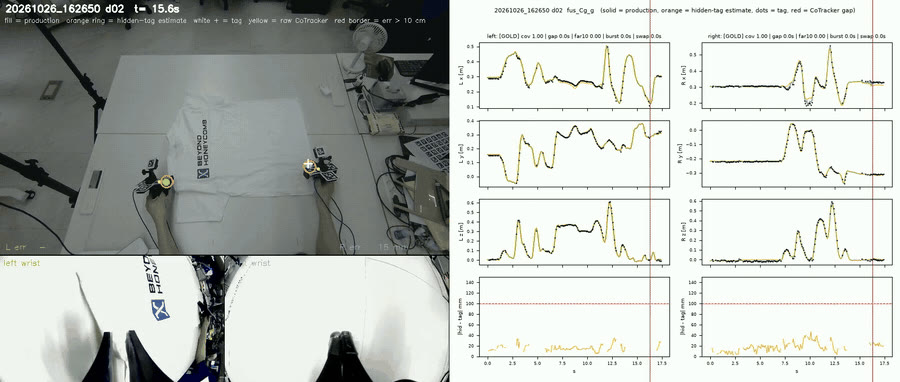
\includegraphics[width=0.85\textwidth]{figures/fig_fusion_qa.jpg}
\caption{Per-demo QA video of a GOLD flattening demo. Top left: fixed camera with the fused jaw tips (filled dots), the
estimate made with that marker hidden (orange ring), the marker itself (white +) and raw CoTracker points (yellow).
Bottom left: both wrist cameras. Right: $x$, $y$, $z$ of each hand over time and the hidden-marker error (bottom row; red
dashed line = 10\,cm).}
\label{fig:fusqa}
\end{figure*}

\subsection{What we tried before, and why it failed}\label{sec:slam}
Before Cg, three pose sources were tried. (i) \emph{Wrist-camera SLAM.} MASt3R-SLAM on the wrist fisheye, with
automatic restarts after tracking loss, was accurate where it tracked (2--14\mm on held-out marker frames) but kept only
19--48\,\% of frames and 0--38\,\% of the marker-hidden frames around grasps, and joins between restarted segments jumped
40--73\mm: white cloth fills the view at close range and the hand moves fast. ORB-SLAM3 mono-inertial initialised with
good rotation, but its translation scale diverged by 30--1000$\times$; hand accelerations (median 0.07--0.16\,m/s$^2$)
were below the accelerometer bias (0.25--0.43\,m/s$^2$), so scale was not observable. Stereo VIO with an earlier stereo
camera diverged, and that camera was dropped on 16 October. (ii) \emph{An earlier smoother} (SLAM + external body
tracking + IMU) passed all its own quality checks yet was 4--6\,cm from the jaw position seen by the external camera,
because of a stale camera--IMU rotation (17--24$^\circ$ off), a lever arm that converged 20--35\,cm wrong, and a wrong
anchor; internal residuals could not see them. This motivated the marker rig. (iii) \emph{Markers with IMU fill}, used
for the replay track, leave the grasp phases interpolated (about a fifth of the right-hand frames of the replayed demo).
The code of (i) and (ii) is in \code{legacy/}.

% =====================================================================
\section{Jaw Labels}\label{sec:jaw}
\textbf{From the wrist video (demonstrations up to 28 October).} An ImageNet-pretrained ResNet-18~\cite{he2016resnet} per
hand classifies a fixed crop of the wrist fisheye that shows the jaws, with hysteresis on its output. Since 22 October a
YOLO-pose keypoint model finds the two jaw tips, and their distance gives a continuous aperture $g$ (0 closed, 1 open);
it agrees with hand labels on 100\,\% (left) and 98\,\% (right) of frames of a re-angled take.

\textbf{From the servo (demonstrations since 29 October).} The torque-off servo is read at about 100\,Hz on the same host
clock as the cameras. Its position is mapped through a per-hand calibration (closed \ldots{} open ticks) to $g$, then to
open/close events with hysteresis and a minimum dwell. The reading is re-centred per recording, because unplugging or
power-cycling a servo shifts its whole range; the recorder warns aloud when a servo reads outside its calibrated range.
The output has the same format as the video labels, so every later stage is unchanged.

\textbf{Never mixed.} On recordings that have both, the video classifier agrees with the servo on only about 70--80\,\% of
frames (per frame, on the servo-equipped takes). Video- and servo-derived labels are therefore kept apart and never mixed in one comparison or training set. A
model trained to reproduce the servo from the wrist video, for relabelling older demonstrations, was evaluated; a
candidate dataset built with it on 31 October has not been used for any reported model.

% =====================================================================
\section{Replay Track: Converted Demonstrations on the Robot}\label{sec:replay}
The replay track (8--22 October) converted one demonstration into a robot trajectory and replayed it open loop. It used
the marker pose with IMU fill and video jaw labels, and is kept here because its measurements are the evidence that the
calibration and conversion are geometrically sound.

\subsection{Conversion and execution}
\emph{Robotization} changes the human path only by continuous warps, never by clipping: a lateral compression toward each
arm's own side with a softplus ceiling at the midline (minimum separation 0.06\,m) and a softplus floor above the table;
every frame stores its displacement and a quality class (thresholds 20 and 50\mm). \emph{Planning} uses
joint-limit-aware differential IK (Pink) with position prioritised over orientation, a bound of 5$^\circ$ per frame on
each joint, wrist-roll relaxation about the tool axis, the jaw's 180$^\circ$ symmetry, and a finger-corner clearance
model; jaw commands are issued early by the measured jaw latency (open 320\,ms, close 480\,ms). \emph{Safety checks} run
offline before anything moves: IK error, joint limits and speed, TCP and link heights above the table, and at least
120\mm between the links of the two arms. Commands stream at 30\,Hz to the 100\,Hz bridge; at 0.35$\times$ speed a 33\,s
demo takes 94\,s.

\textbf{Metrics.} Three levels are compared in $B$ on the host clock: A the human jaw tip, B the robot command (FK of the
commanded joints) and C the robot (FK of the encoders). A is taken relative to the start of the window, B and C relative
to their first sample, and C is shifted by the lag in 0--1.5\,s that best matches B, so a pure delay is not error. We
report position RMSE and p95, the geodesic rotation error, the amplitude ratio (C over A), C$-$B (tracking) and B$-$A
(what conversion and planning changed). Single-arm gates: RMSE $<$20\mm, p95 $<$30\mm, rotation median $<$5$^\circ$ and
p95 $<$10$^\circ$, amplitude ratio 0.9--1.1. \emph{Relative metrics hide constant offsets}; absolute placement was checked
by tape and video.

\subsection{Results}
\textbf{Single-arm parity.} Six-direction translation strokes: 16/18 pass, median per-axis RMSE 5.5--11.6\mm (max
14.5\mm), endpoint repeatability $\le$8\mm; one failure was a marginal cross-axis leak, the other a poor human stroke.
Rotation strokes: amplitude ratio 0.98--1.04, median error 0.3--1.6$^\circ$. Free combined motion near human speed: 2/2
pass (RMSE 13.7 / 14.6\mm, p95 26 / 29\mm, rotation median 1.7 / 1.4$^\circ$, robot lag about 0.2\,s). B$-$A was at most
3.4\mm, so the residual was robot tracking, not conversion. The robot jaw command fell within 0.5\,\% of window progress of
the human jaw event.

\textbf{Controller finding.} The moving error did not change when the proportional gain was raised. With an
integral-only feed-forward $\tau_\mathrm{ff}[k{+}1]=\tau_\mathrm{ff}[k]+K_i e[k]\Delta t$ and no gravity model, a
quasi-static analysis of $\tau_g=K_p e+\tau_\mathrm{ff}$ gives a moving error $e\approx\dot\tau_g/K_i$, independent of
$K_p$; a simulation explained 77\,\% of the measured shoulder-joint error. Raising $K_i$ in two steps reduced the
forward-stroke RMSE from 25--37\mm to 12--14\mm (earlier settings had passed 0/6, 3/6 and 5/6 strokes).

\textbf{First cloth grasp.} After the TCP correction, one arm replayed the grasp window of a demonstration and picked up
and lifted the T-shirt. The first attempt scraped the table at a strongly tilted tool, which led to the finger-corner
clearance model.

\begin{figure*}[!t]
\centering
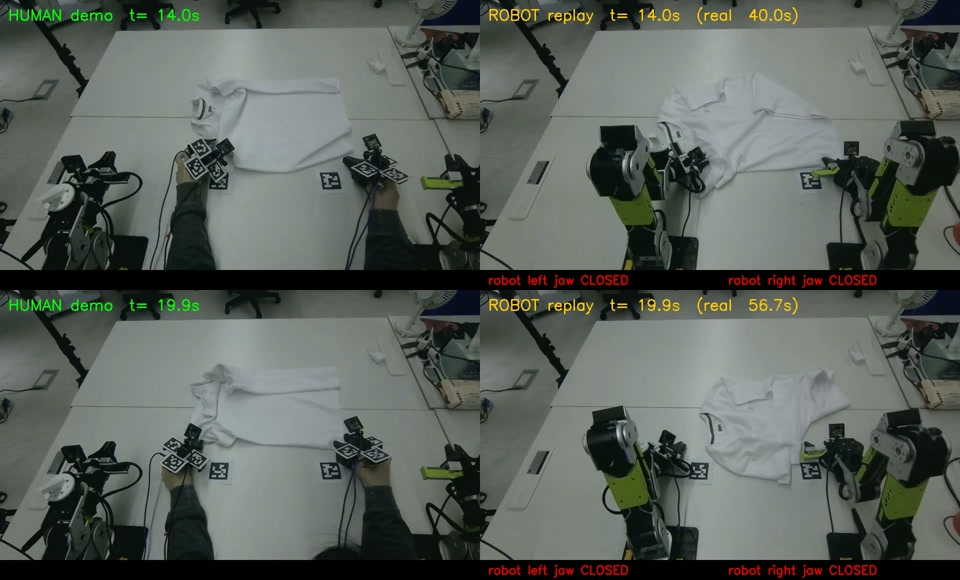
\includegraphics[width=0.85\textwidth]{figures/fig_sidebyside.jpg}
\caption{Human demonstration (left) and two-arm robot replay of the converted trajectory (right), filmed by the same
fixed camera and aligned on one clock (robot at 0.35$\times$). The bars show the robot jaw commands. The jaws hold the
shirt edge and drag it; the shirt is moved, but not folded as by the human.}
\label{fig:sbs}
\end{figure*}

\textbf{Two-arm replay of a full demonstration.} One 33\,s demonstration was replayed at about a third of human speed
(94\,s; Fig.~\ref{fig:sbs}). In its window the right hand had a visible marker in 79\,\% of frames and the left in
95\,\%; 21\,\% of the right-hand frames were interpolated. The robotization displacement had a p95 of 9.3\mm (right) and
20.6\mm (left). The plan kept the IK error within 6.3\mm / 11.5$^\circ$ (right) and 10.3\mm / 21$^\circ$ (left), and the
arms stayed at least 27\,cm apart. Table~\ref{tab:rep} gives the error of four runs with one unchanged plan, against the
robotized path that was replayed. The runs agree within about 1\mm: the robot is deterministic and the remaining error
is systematic. Against the raw human path the RMSE is about 22\mm (right) and 32--34\mm (left), because the robotization
displacement then also counts as error. The left command already deviates more from the replayed path (B$-$A 22.6\mm vs
8.6\mm): the left IK gives up more orientation.

\begin{table}[t]
\caption{Two-arm replay, range over four runs with one plan (whole demo as one window; reference = robotized path)}\label{tab:rep}
\centering\small
\begin{tabular}{@{}lcc@{}}
\toprule
 & right & left \\
\midrule
position RMSE & 17.2--17.4\mm & 29.0--30.3\mm \\
position p95 & 35--37\mm & 50--51\mm \\
rotation median & 8.1$^\circ$ & 12.3--12.7$^\circ$ \\
rotation p95 & 12.6--12.7$^\circ$ & 17.0--17.2$^\circ$ \\
C$-$B (tracking) & 12.1--12.3\mm & 14.5--15.5\mm \\
B$-$A (conversion, IK) & 8.6\mm & 22.6\mm \\
\bottomrule
\end{tabular}
\end{table}

\textbf{Jaw height at grasp.} With a conservative finger-corner clearance the jaws closed 19--61\mm above the table and
missed the cloth. Allowing the finger corner to touch the table plane, as human fingers do, brought the closes to
14--16\mm (right, 4 closes) and 5--19\mm (left, 5 closes) above the table, within 2--8\mm in $xy$ of the command at that
moment; the human closes at about 10\mm (Fig.~\ref{fig:close}). Tilting the tool toward vertical instead failed (the IK
could not follow even 15$^\circ$; errors up to 100\mm), and closing at the lowest nearby point, a heuristic, was rejected.

\begin{figure}[!t]
\centering
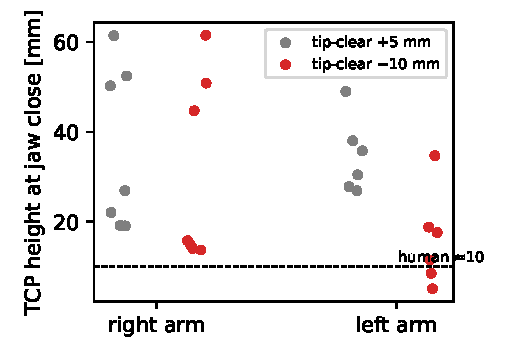
\includegraphics[width=0.62\columnwidth]{figures/fig_close_height.pdf}
\caption{TCP height at each jaw close with the conservative finger-corner clearance and with the corner allowed to
touch the table plane. Dashed line: the human ($\approx$10\mm).}
\label{fig:close}
\end{figure}

\textbf{Outcome.} In two runs the shirt lay 15--20\,cm farther away than in the demonstration and the jaws closed on the
empty table. In one run the jaws caught the shirt edge and dragged it; the shirt was moved, but not folded as by the
human. Open-loop replay needs the cloth where the human's was; the next step is therefore a policy that sees the cloth.

% =====================================================================
\section{Policy Training Data}\label{sec:data}
\textbf{Collection.} 318 demonstrations of \emph{flattening} a crumpled T-shirt were recorded on 26 and 27 October; 300
were successful (beige 72, black 92, white 82, blue 54), judged on the frame 0.5\,s before each demo ends. The camera
sits at 113\,cm so that both hands stay in view. Each gripper track is assigned to an arm by its side of the table,
because the rig labels on the 22 October and later takes were found swapped against the wrist cameras.

\textbf{Trims.} The waiting start and the still end would be learned as actions. Each demo is cut to 0.3\,s before the
first and 0.3\,s after the last moment either hand moves faster than 10\,cm/s. A one-hand tracking gap of at least 0.8\,s
that starts within 0.5\,s of the window start (or ends within 0.5\,s of its end) is cut away instead of grading the demo
down, unless less than 8\,s would remain.

\textbf{Grades.} A demo is \textbf{GOLD} if both arms have coverage $\ge$0.95, no gap over 1\,s, at most 0.05 of valid
frames more than 10\,cm from a visible marker, no such burst over 0.5\,s, no hand-swap frames, a clean first second and
no gap of 1\,s or more within $\pm$1\,s of a jaw event; \textbf{REJECT} if any arm has a gap over 3\,s, coverage below
0.80, more than 0.20 of frames far off, a burst over 2\,s or swaps over 1\,s; otherwise \textbf{SILVER}. Whole demos are
kept or dropped. Of the first 139 graded demos, 133 are GOLD, 5 SILVER and 1 REJECT. The flattening fine-tunes use 281
GOLD demos from all 300; the final grade counts over all 300 are not reported here.

\textbf{Labels before IK.} The earlier label B was the IK$\to$FK of the robotized path. IK makes execution choices
(wrist-roll relaxation, a 180$^\circ$ tool flip near joint limits, pushes that keep the arms apart) and bakes them into
the data, and it moved the target most exactly where it matters: on the first 139 demos (about 123k arm-frames) IK$\to$FK
moves the target by p95 $\approx$53\mm overall and $\approx$58\mm at grasps (Table~\ref{tab:ikqa}). On the same demos
20.3\,\% of frames need a large IK correction, mostly from execution choices, and 0.8\,\% are truly out of reach (hands
lifted far above the table). The label is therefore the Cartesian jaw-tip pose before IK, stored absolute in $B$; IK is
a checker offline and the executor online, and B is kept for QA only. With labels F and A the IK result changes no value
and masks no frame; a demo is dropped only if IK cannot be run on it at all.

\begin{table}[t]
\caption{IK check of the Cartesian label (first 139 demos). ``Large'' = IK position error $>$30\mm or rotation
$>$30$^\circ$; causes assigned in order, first match wins.}\label{tab:ikqa}
\centering\small
\begin{tabular}{@{}lccc@{}}
\toprule
 & all & left & right \\
\midrule
IK$\to$FK vs Cartesian, position p95 & 53\mm & 70\mm & 28\mm \\
frames with a large correction & 20.3\,\% & 27.8\,\% & 12.9\,\% \\
\quad wrist-roll relaxation & 7.6\,\% & 14.8\,\% & 0.4\,\% \\
\quad other (IK lag) & 4.1\,\% & 5.9\,\% & 2.3\,\% \\
\quad joint limit & 3.2\,\% & 2.9\,\% & 3.5\,\% \\
\quad tool flip & 3.1\,\% & 1.3\,\% & 4.9\,\% \\
\quad workspace / table & 0.8\,\% & 0.9\,\% & 0.7\,\% \\
\quad out of reach & 0.8\,\% & 1.3\,\% & 0.4\,\% \\
\quad arm spacing & 0.6\,\% & 0.6\,\% & 0.6\,\% \\
\bottomrule
\end{tabular}
\end{table}

\textbf{Label F: no clamp (29 October).} Label A was the fused jaw-tip pose in reBot gripper axes, smoothed over
0.25\,s, plus a table-clearance step (tilt toward vertical up to 30$^\circ$, then a lift of the finger corner). That step
lifted 44\,\% of label frames, by 27\mm at the median (max 65\mm), so a policy could not learn to go down to the cloth
(Sec.~\ref{sec:policy}). The current label F is the same pose without the clearance step: smoothed over 0.25\,s, no
clamp, lift or feasibility edit; IK does not change or mask it. Limits belong to deployment, not to training labels.

\textbf{Time stretch.} Human demonstrations are faster than the arms can follow (jaw tip p95 0.93\,m/s, 127$^\circ$/s).
Time-stretched copies of the data set resample pose, jaw events and every camera frame (nearest source frame) on one
common slower timeline: with a factor $s$, rows stay at 20\,Hz but advance $s\cdot$0.05\,s of source time, so a
demo becomes $1/s$ times longer: 0.3$\times$ for the flattening set, 0.5$\times$ for the pinching sets.

\textbf{Dataset.} LeRobot v3 at 20\,Hz with three cameras (fixed camera and both wrist cameras), a 30-D state (per-arm
pose relative to the episode start, both jaws, the left--right relative pose) and a 20-D absolute action (per arm
position and 6-D rotation, then both jaws; the jaw target is the binary jaw state with a 0.1\,s ramp) with a
per-dimension mask. The policy learns relative
motion $T_t^{-1}T_{t+k}$, $k=1\ldots32$, built in the training loader.

% =====================================================================
\section{First Policies on the Robot}\label{sec:policy}
\textbf{Deploy loop.} Each cycle takes fresh images and the measured joints; FK gives the current TCP; the policy
predicts 32 relative steps; the newest TCP re-anchors the chunk (latency); a limiter bounds speed and the table floor;
Pink IK solves the joints; safety checks (workspace, link-to-link capsules, table, joint limits) must pass; only the first
steps of each plan are committed before re-planning (4 by default for the DiT; Fig.~\ref{fig:deploy}). On 27 October a bridge restart without
the jaw-opening limit let one jaw open to the end of its travel and break its holder; deployment now refuses to send
commands unless the bridge reports the jaw limits.

\begin{figure}[!t]
\centering
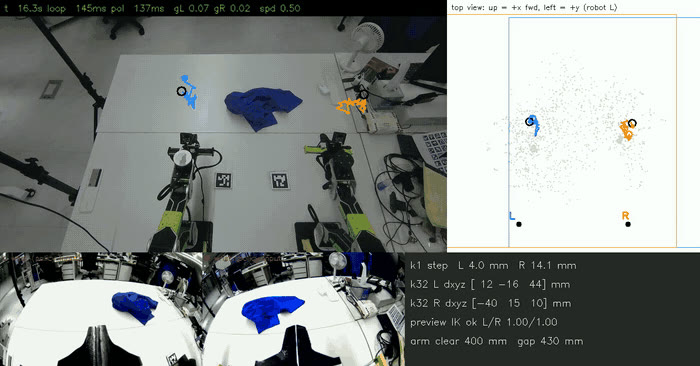
\includegraphics[width=\columnwidth]{figures/fig_deploy_ui.jpg}
\caption{Deploy UI in a dry run (no command sent): predicted 32-step jaw-tip paths on the fixed camera (left blue, right
orange), top view in the robot base, both robot wrist cameras and the live checks.}
\label{fig:deploy}
\end{figure}

\textbf{Policies.} (1) A diffusion-transformer policy (DiT, CLIP~\cite{radford2021clip} text, 2 observation frames,
horizon 33) pretrained for 300k steps on the public Soft-Fold cloth-folding data ran on the robot in dry runs without
safety violations. The DiT fine-tunes on our data start from a DiT pretrained for 100k steps on a 1\,:\,1\,:\,1 mix of
Soft-Fold, iPhUMI~\cite{iphumi} and PrimeBot UMI~\cite{primebot}. (2) The X-VLA base model~\cite{xvla} pretrained on a
1\,:\,1\,:\,1 mix of the same three datasets, one domain prompt per source. Both were fine-tuned on 281 GOLD flattening
demos (from late October) and run with the receding-horizon loop. What is known from these runs is qualitative: the
arms approach the cloth but stop short of it and close the jaws early. The trials were not counted, and for the runs of
28--31 October the checkpoints, label kinds and speeds were not recorded. \textbf{No success rate is reported.}

\textbf{Causes and data problems.} Two causes were recorded from the robot runs: the jaw-state copying and the
wrist-camera placement (first and last rows of Table~\ref{tab:causes}). The other three rows were found afterwards by
checking the labels. All but the camera re-mount are changed; re-mounting the robot wrist cameras is next.

\begin{table}[t]
\caption{What the first policies exposed in the data (28 October -- 1 November)}\label{tab:causes}
\centering\small
\begin{tabular}{@{}>{\raggedright\arraybackslash}p{0.45\columnwidth}>{\raggedright\arraybackslash}p{0.47\columnwidth}@{}}
\toprule
finding & change \\
\midrule
Jaw closed early and never re-opened: the policy copied the jaw state from its observation input & jaw state masked to 0 in the observation, in training and deploy \\
Table clearance in the label lifted 44\,\% of frames by 27\mm (median) & label F: fused jaw tip, no clamp (Sec.~\ref{sec:data}) \\
Demos faster than the arms (p95 0.93\,m/s, 127$^\circ$/s) & time-stretched copies, 0.3$\times$ / 0.5$\times$ \\
Video jaw labels disagree with the true aperture & servo encoder labels since 29 October; never mixed (Sec.~\ref{sec:jaw}) \\
Robot wrist cameras tilted 11--13$^\circ$ less toward the tool axis and 25--44\mm closer than the hand-worn ones (table-tag PnP) & re-mount to the hand-worn geometry (next) \\
\bottomrule
\end{tabular}
\end{table}

Also added and \emph{not yet validated on the robot}: a real-time-chunking blend between plans (the UI default since
29 October; whether it was on in a given robot run was not recorded) and an X-VLA policy server.

% =====================================================================
\section{Pinching Feasibility Test (first robot grasps)}\label{sec:pinch}
To separate ``the pipeline cannot teach a grasp'' from ``flattening is too hard for this amount of data'', the first
robot feasibility test was reduced to one sub-skill: \textbf{pinch one sleeve with the left hand}. The right arm is idle
in all data; in the robot runs of 2 November both arms were under policy control and the right arm stayed at its start
pose.

\begin{figure*}[!t]
\centering
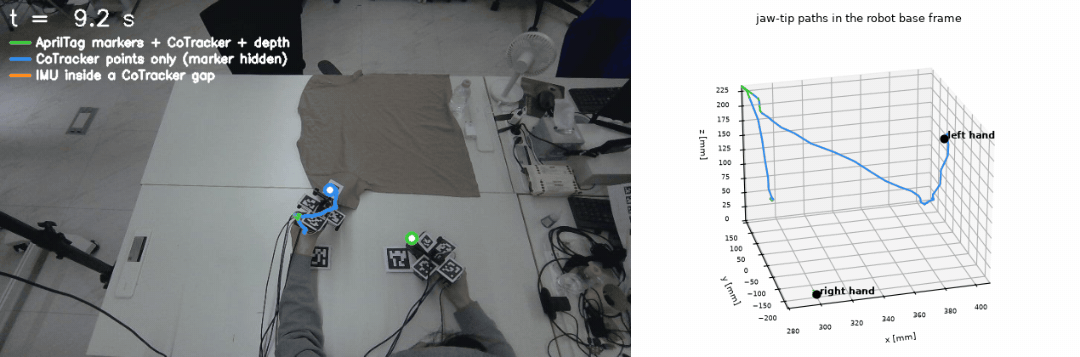
\includegraphics[width=0.85\textwidth]{figures/fig_pinching_cg.png}
\caption{A GOLD pinching demonstration recorded on 1 November: Cg jaw-tip paths coloured by the source of each frame
(green: a gripper marker visible; blue: point tracking only, marker hidden; orange: IMU inside a tracking gap). Left:
projected into the fixed camera; right: both hands in the robot base frame. The right hand stays at its start marker.}
\label{fig:pinch}
\end{figure*}

\textbf{Data.} All sets use the Cg trajectory source (Fig.~\ref{fig:pinch}) with label F, servo jaw labels and the
0.5$\times$ time stretch, and keep GOLD and SILVER demos (Table~\ref{tab:pinch}). An earlier trajectory source (A$'$, one
position bias per demo and arm from the tags of the first 2\,s) had NaN spans inside some demos of 1 November, and IK
failed on 4 of them, so every set was rebuilt from Cg; the two sources are never mixed. On 1 November the gate kept 147
demos; the dataset converter dropped 3 whose trimmed window was shorter than 5\,s, so with the 53 of 30 October the
training set has 197 demonstrations (53 + 144; 62,160 frames).

\begin{table}[t]
\caption{Pinching data, status of 1 November (kept = GOLD or SILVER; built = episodes in the dataset)}\label{tab:pinch}
\centering\small
\begin{tabular}{@{}lcccc@{}}
\toprule
recorded & takes & demos & kept & built \\
\midrule
30 October & 5 & 74 & 53 & 53 \\
1 November, T1 + T2 & 2 & 60 & 56 & 55 \\
1 November, T3 & 1 & 35 & 33 & 33 \\
1 November, T4 & 1 & 10 & 10 & 10 \\
1 November, T5 & 1 & 50 & 48 & 46 \\
\bottomrule
\end{tabular}
\end{table}

\textbf{Test sets (never trained on).} P20: 19 demonstrations (6207 frames) from two held-out takes, for arm and jaw:
all 10 demos of the 30 October take, not gate-filtered, and 9 of the 10 of the 1 November take (the tenth was
rejected). A reject set: every 1 November demo the quality gate rejected, used for jaw timing only,
because its servo jaw label is valid and its arm label is not.

\textbf{Model.} The DiT fine-tuned on the 53 demos of 30 October (trajectory source A$'$, label F) is the starting point
and the baseline; on P20 built from Cg it scores 19.89\mm (\code{val_score_mm}: the mean, over $k=16$ and $k=32$ and
over the left and right arm, of the translation deviation, position only; 19.13\mm on P20 built from source A$'$). Its score on the 10 demos of P10 had plateaued at 17.1--17.7\mm
since about 150 epochs. A fine-tune from these weights on the merged 197-demo Cg set, with a new optimizer and a cosine schedule
over 500 epochs, a checkpoint every 25 epochs, gradient clipping off, a jaw BCE head and new train-time image
augmentation, started on 1 November (about 4.7 days planned). On P20 its checkpoints after 25 and 50 epochs score
17.29 and 18.89\mm{} (baseline 19.89\mm); the 50-epoch checkpoint is the one that grasped on the robot, so the offline
score did not pick the robot checkpoint. Earlier in this chain, a DiT
pretrained on the three-dataset mix was fine-tuned on the flattening GOLD demos (label F, 0.3$\times$) and then on
pinching data, before the 30 October set.

\textbf{Robot-side changes.} Per-arm table-height calibration from jaw-tip touches on the table tags (plane tilt
4.9$^\circ$ left, 2.6$^\circ$ right), added to every committed command when the UI option is on; the fixed camera, which had moved since
26 October, re-aimed to its earlier view (residual about 5\,px / 0.4$^\circ$); and a soft stop that brakes on the current
command without latching an emergency stop.

\textbf{Robot runs of 1 November (qualitative, not counted).} Two DiT checkpoints were run with 32 steps committed per
plan and speed 1 (later 1.5): the flattening fine-tune on 281 GOLD + 48 servo-labelled demos (label F, 0.3$\times$; two
runs of about 70\,s) and the pinching baseline (one short run). In both the left jaw was mostly commanded open and the
right jaw stayed closed; in the first run the left wrist had one motor fault and the left arm once lagged its command by
more than 20$^\circ$. No success or failure was scored.

\begin{figure*}[!t]
\centering
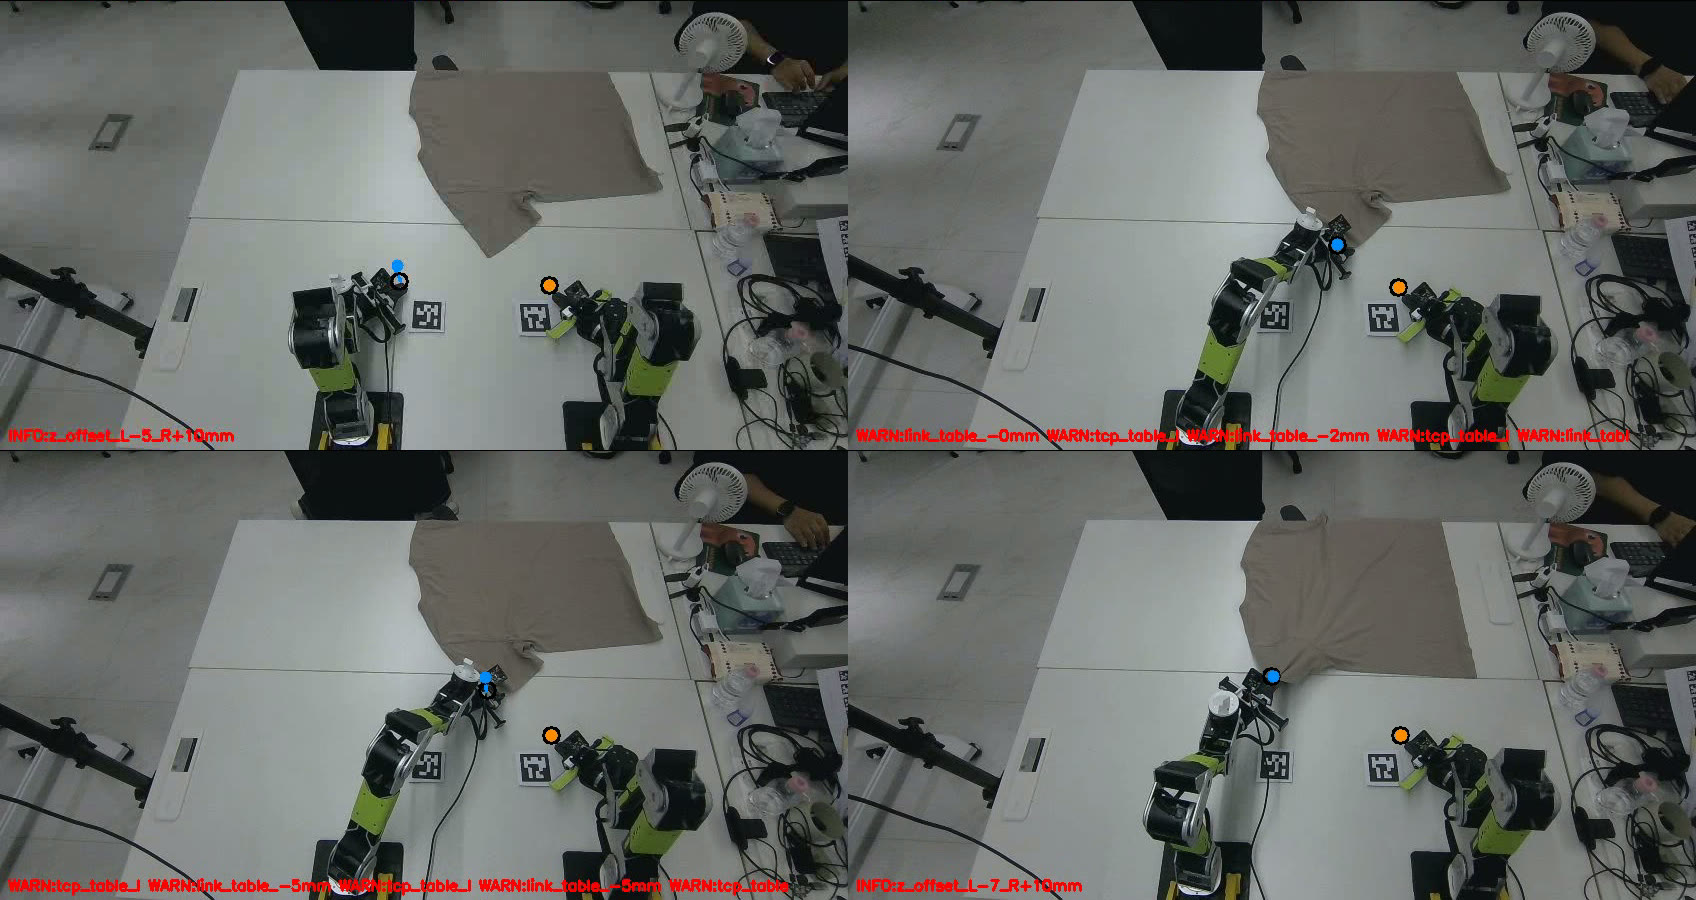
\includegraphics[width=0.85\textwidth]{figures/fig_pinching_robot_1102.jpg}
\caption{One of the real-robot runs of 2 November judged successful by the operator (50-epoch checkpoint; fixed camera,
one frame per plan cycle; trials were not counted). Top left: start; top right: the left arm approaches the sleeve
end with the jaw open (7\,s); bottom left: jaw closed on the sleeve (11\,s); bottom right: the sleeve pulled (22\,s).
Blue / orange dots: the policy's next targets for the left / right jaw. Red text: the deploy loop's table-proximity
messages.}
\label{fig:pinchrobot}
\end{figure*}

\textbf{Robot runs of 2 November (first grasps; trials were not counted).} The 50-epoch checkpoint of the 197-demo
fine-tune was run with 32 steps committed per plan, speed 1, real-time-chunking look-ahead off, 10 DDIM sampling steps,
per-arm height calibration on and the soft stop. Successful grasps of the sleeve were observed in real-robot trials on
2 November (Fig.~\ref{fig:pinchrobot}): the left arm approaches the sleeve end with the jaw open, closes on it and pulls
it. The trials were not counted, so no success rate is given. After a miss the policy grasps elsewhere instead of
retrying: the data contain no recovery demonstrations, so post-failure states are out of distribution. A retry means
sending the arms back to the start pose and starting again; the data fix is to record recovery demonstrations.
Hardware changes that day: the arms' USB locations had swapped after re-cabling (fixed in the launch configuration);
the left jaw has mechanical slack and now closes 25$^\circ$ past its zero, with the extra squeeze ramped in over the
last 30$^\circ$ of travel; the start move now closes both jaws (a parked jaw relaxes open); one robot wrist camera
stalled once and the deploy UI was restarted.

\textbf{Status: first grasps observed, trials were not counted.} Robot trials will be reported with the number of trials
and successes, whatever the outcome.

% =====================================================================
\section{Flattening after the Pinching Test (2--5 November)}\label{sec:flat}
After the first pinching grasps the work returned to flattening, with both hands, Cg trajectories and servo jaw labels.
The numbers of this section are in \code{docs/status_2026-11-05.md}.

\textbf{FLAT149: the UMI recipe.} 149 flattening demonstrations (48 of 30 October and 101 of 2 November; a demo was kept
only if the shirt ended flat in the fixed-camera frame) were built at 0.5$\times$ speed with a continuous jaw target.
Training followed the cloth-folding recipe of the UMI appendix~\cite{chi2024umi} item by item: 100 epochs, learning rate
$3\cdot10^{-4}$ (vision encoder $3\cdot10^{-5}$), DDIM with 50 training and 16 inference steps, and image augmentation
matching UMI's random crop (zoom 0.05, shift 0.025), rotation ($\pm5^\circ$) and colour jitter (brightness 0.3,
contrast 0.4, saturation 0.5, hue 0.08). The jaw is learned as a continuous value (no BCE head) and binarised at
deployment. Training started from the H100 checkpoint of the GOLD-281 flattening fine-tune and ran on four H100s. The
hue shift is a rotation of the chroma plane in YIQ space (one $3\times3$ matrix): the library hue adjustment cost about
62\,ms per camera sample on the CPU data workers and made the run data-bound at about 3\,s per update. On the held-out
sets the best validation checkpoint is at epoch 80 (\code{val_score_mm} 60.89) and the best test checkpoint at epoch 90
(64.36). No counted robot result exists.

\textbf{Deploy changes (3 November).} A motion-amplitude scale (\code{amp}) shrinks each committed step's translation
and rotation about the current pose (the user found the motion too large); the start move can use the medoid start of
any dataset (\code{start_root}; the FLAT149 starts lie 19 / 31\mm (left / right) from those of GOLD-281); a
camera-alignment tool compares the live view with a reference day.

\begin{figure*}[!t]
\centering
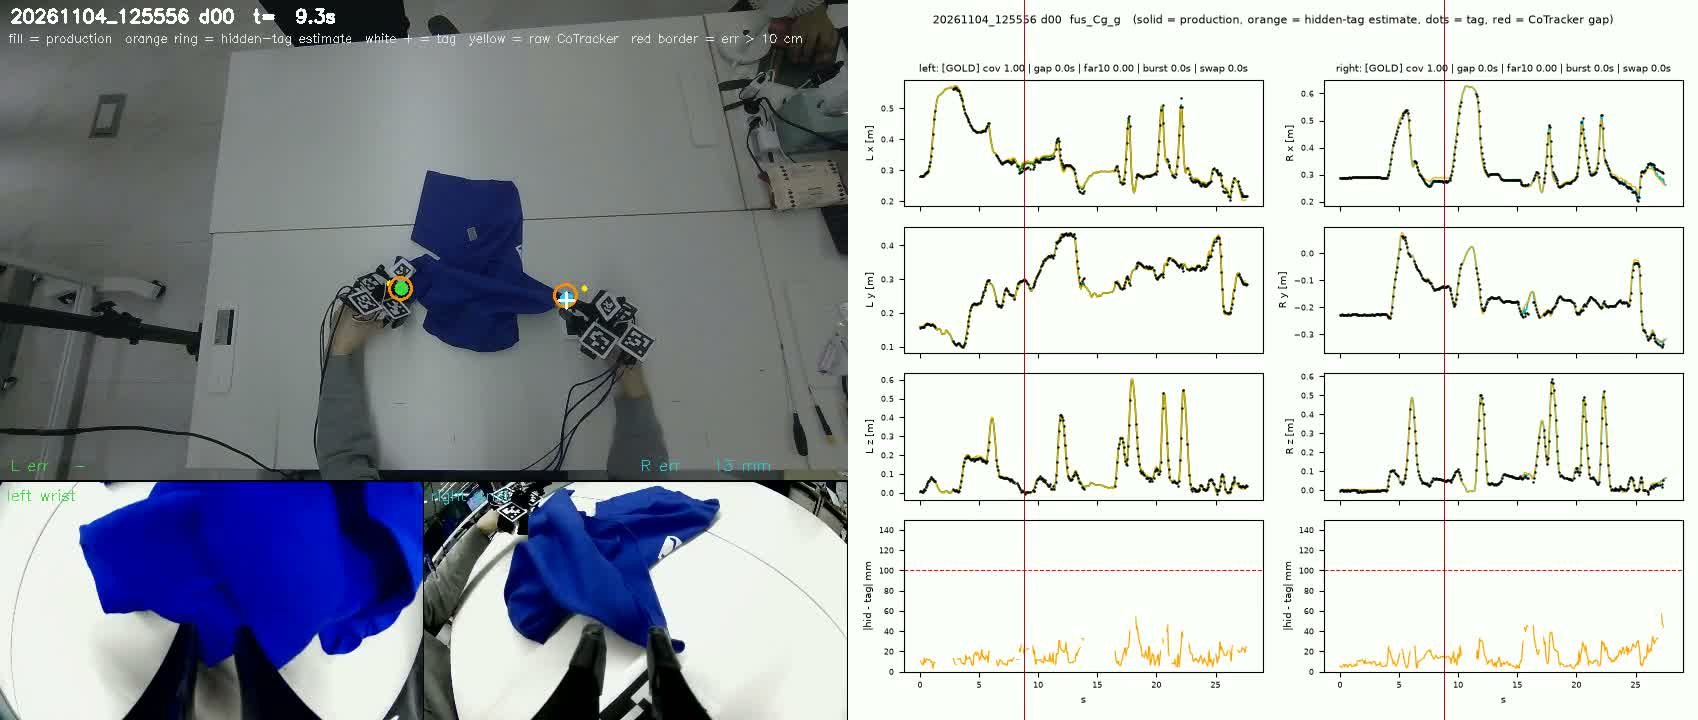
\includegraphics[width=0.95\textwidth]{figures/fig_fusion_qa_1104.jpg}
\caption{Per-demo QA video of a GOLD flattening demo under the re-aimed camera (4 November, train split). Top left: fixed
camera with the fused jaw tips (filled dots), the estimate made with that marker hidden (orange ring), the marker itself
(white +) and raw CoTracker points (yellow). Bottom left: both wrist cameras. Right: $x$, $y$, $z$ of each hand over time
and the hidden-marker error (bottom row).}
\label{fig:fusqa1104}
\end{figure*}

\textbf{Camera re-aimed, new collection, split by tracking gaps (3--4 November).} The fixed camera was re-aimed during a
take on 3 November; that take and later ones use a re-solved calibration from the two table anchor tags and the table
plane (the two coplanar tags make the PnP initialisation ambiguous, so every IPPE solution is tried and the one with the
camera highest above the table is kept), and are kept apart from earlier data. On 3 November 7 takes with 100
demonstrations were recorded (Fig.~\ref{fig:fusqa1104}). Every demo is trimmed at both ends (both arms slower than
3\,cm/s for 0.5\,s, margin 0.3\,s), and the longest point-tracking gap is measured \emph{inside} the trimmed window:
\textbf{train} = GOLD with a longest gap below 0.25\,s; GOLD with a longer gap alternates between \textbf{validation}
and \textbf{test}; SILVER without any gap also goes to train, other SILVER and REJECT form separate sets for auxiliary
evaluation and analysis. Datasets are built at
0.3$\times$ with label F and the continuous jaw; timelines and images are never cut. Positions inside a tracking or marker
gap of at least 0.3\,s are masked in the loss, and once one future step of a predicted chunk is masked, every later step
of that chunk is masked too, because the path across a gap is uncertain.

\begin{table}[t]
\caption{FLAT250: offline score (val\_score\_mm) per epoch, mm, lower is better (stride 16)}\label{tab:flat250}
\centering\small
\begin{tabular}{@{}lcc@{}}
\toprule
epoch & validation & test \\
\midrule
0 (initial checkpoint) & 71.67 & 72.27 \\
1 & 102.36 & 101.78 \\
4 & 82.81 & 82.42 \\
8 & 60.74 & 59.85 \\
10 & 57.64 & 56.95 \\
12 & 53.56 & 54.16 \\
13 & 52.56 & 52.32 \\
\bottomrule
\end{tabular}
\end{table}

\textbf{FLAT250 (4--5 November).} The per-take sets of 3 and 4 November were aggregated into 250 training demonstrations
(444217 frames), 39 for validation and 38 for test, and trained with the FLAT149 recipe (global batch 1024, 100 epochs)
on two RTX 4090 GPUs with distributed data parallel, saving a checkpoint every epoch. Every epoch is evaluated offline on
both held-out sets (Table~\ref{tab:flat250}): the score first rises, then falls below the initial checkpoint from
epoch 6 on (validation). The run was stopped after epoch 13, its best checkpoint, to free the GPUs for the run below;
epochs 8 and 10--13 were copied to the robot computer as rollout candidates; no counted robot result exists.

\textbf{Does the closed jaw hold the cloth? (5 November).} The jaw servo is read with torque off, position only: it has no
load or current signal, and the closed position does not separate cloth from nothing. The cue therefore comes from the
wrist camera. Jaw close events of 343 flattening demos were segmented with a tighter hysteresis for this purpose (which
uncovered 148 partial re-opens hidden in the earlier segmentation); the user labeled 585 events blind to any prediction
over four rounds, of which 543 map onto the new events (372 held, 171 empty). A ResNet-18 on a crop around the jaw tips
of the wrist image reaches, in take-grouped 5-fold cross-validation, per-event F1 0.90 for held and 0.78 for empty. A
causal per-frame probability $p_\mathrm{grasp}(t)$ at 15\,Hz (mean over the last 0.4\,s, restarted at every jaw state
change) has a median of 0.99 on held and 0.03 on empty events; 12\,\% of held events dip below 0.2 and 17\,\% of empty
events touch 0.9 at least once. A frozen generator writes $p_\mathrm{grasp}$ for every frame of a dataset. A new run
with the same recipe feeds it into the (otherwise masked) jaw slots of the observation state, on the data of 3, 4 and 5
November (301 training, 46 validation and 45 test demonstrations); after two epochs its offline score is 68.79 /
68.43 (validation / test; other held-out sets than FLAT250). The deploy loop does not compute $p_\mathrm{grasp}$ yet.

% =====================================================================
\section{Superseded Approaches}\label{sec:superseded}
\begin{table*}[t]
\caption{Current pipeline and what it replaced}\label{tab:superseded}
\centering\small
\begin{tabular}{@{}>{\raggedright\arraybackslash}p{0.11\textwidth}>{\raggedright\arraybackslash}p{0.36\textwidth}>{\raggedright\arraybackslash}p{0.30\textwidth}>{\raggedright\arraybackslash}p{0.16\textwidth}@{}}
\toprule
part & current (1 November) & replaced & why \\
\midrule
Pose source & CoTracker3 on the fixed camera + marker anchors + constant bias, IMU only in gaps (Cg) & MASt3R wrist-SLAM gap
filler; ORB-SLAM3; stereo VIO; SLAM + body-tracking smoother; markers + IMU fill (replay track) & lost at grasps; scale
unobservable; 4--6\,cm label error \\
Camera $\leftrightarrow$ robot & re-solved after every camera move from two table tags + the table plane & one 32-pose
robot-held-marker solve & camera raised so both hands stay in view \\
Jaw state & servo encoder (since 29 October); video model for older demos & red-tape jaw detector (tape removed
20 October) & detector fired on background; video labels disagree with the servo \\
Arm assignment & by the gripper's side of the table & by rig label & labels swapped \\
Label & F: fused jaw-tip pose (gripper axes, 0.25\,s smoothing) before IK, no clamp & B: IK$\to$FK; A: with table clearance & IK choices and the clamp
moved the target at grasps \\
Data speed & 0.3$\times$ / 0.5$\times$ time-stretched copies & human speed & too fast for the arms \\
Execution & receding-horizon deploy, 4 steps per plan (DiT default) & whole-demo open-loop replay & replay needs the same scene \\
\bottomrule
\end{tabular}
\end{table*}

Table~\ref{tab:superseded} lists what was replaced, when the current pipeline was built, and why. The code of dropped
approaches is in \code{legacy/}, with a README table of dates and reasons.

% =====================================================================
\section{Lessons}\label{sec:lessons}
\begin{enumerate}
\item \emph{Markers plus a fixed camera beat wrist SLAM for contact-rich hand motion.} The failure regime of SLAM (close
  range, textureless cloth, fast motion) is exactly the grasp.
\item \emph{Anchor, do not replace.} Point tracking covers the hidden phases, and the markers remove its absolute error;
  neither is enough alone.
\item \emph{Measure in the world, not in the model.} The 89\mm TCP error and the 70\mm base error were invisible to
  FK-based checks; tape, camera and cloth found them. The 4--6\,cm error of the earlier smoother was invisible to its own
  residuals.
\item \emph{Fix the conversion, do not add heuristics.} Lifting the jaws for clearance cost the grasp; allowing contact
  restored it.
\item \emph{Do not let the executor, or a safety limit, write the label.} IK choices and a table clamp are right for
  execution and wrong as training targets.
\item \emph{One clock for everything.} It made camera, IMU, servo and robot alignment, and side-by-side videos, possible
  without synchronisation hardware.
\item \emph{Model the controller.} The tracking error followed $\dot\tau_g/K_i$; changing $K_p$ could not help.
\end{enumerate}

% =====================================================================
\section{Limitations}\label{sec:limits}
\begin{itemize}
\item \emph{No success rate.} Neither replays nor policies were run as counted trials; outcomes are judged by measurement
  and video.
\item \emph{One setup, one demonstrator.} All numbers come from one physical setup and one person; one demonstration was
  replayed in full on both arms, and its 1\mm repeatability shows determinism, not generality.
\item \emph{Relative parity metrics hide offsets.} Absolute placement was checked only by tape at a few poses and by video.
\item \emph{Pose accuracy at grasps.} The hidden-marker error is measured where markers can be hidden, mostly away from
  the grasp; the error inside long tracking gaps is bounded only by the gates.
\item \emph{Grades and IK statistics} reported here were computed on the first 139 flattening demos; the final grade
  counts over all 300 are not reported; success was judged by one person from one frame.
\item \emph{Jaw labels} from the wrist video have no held-out accuracy number on the older demonstrations, and agree with
  the servo on only about 70--80\,\% of frames where both exist.
\item \emph{Offline scores} such as \code{val_score_mm} measure agreement with held-out human motion, not task success.
\item \emph{Grasp labels} come from one labeler; the frozen $p_\mathrm{grasp}$ generator is trained on all labeled
  events, so its output on those events is in-sample.
\item \emph{Hardware.} The left robot wrist connector has dropped out repeatedly.
\end{itemize}

% =====================================================================
\section{Reproducibility}\label{sec:repro}
\textbf{Repository layout.} \code{src/garment_pipeline/}: the training-data pipeline as an installable package (fusion,
gates, trims, grades, labels, LeRobot dataset, DiT trainer, offline evaluation, deploy), run with
\code{python -m garment_pipeline.<stage>.<module>}; \code{src/visual_teleop/}: recorder, jaw classifier, reBot IK, limits,
safety and replay planner; \code{src/rebot_prep/}: shared marker-rig pose code; \code{scripts/pose/},
\code{scripts/retarget/}, \code{scripts/evaluation/}, \code{scripts/deploy/}: calibration, servo jaw labels, replay
robotization, parity scoring and the robot bridge; \code{scripts/flatten_builds/}, \code{scripts/grasp/}, \code{scripts/ray_jobs/}: the flattening split and builds, grasp labels and $p_\mathrm{grasp}$, cluster jobs; \code{src/egogarment/}: small standalone re-implementations of the
trajectory stages that run on the synthetic data in \code{examples/}; \code{configs/}: calibration results and robot
overrides; \code{hardware/umihand/}: the HandUMI build copy with our modifications (upstream Apache-2.0 licence kept);
\code{legacy/}: superseded code; \code{docs/}, \code{media/}, \code{report/}: documentation, media and this report.

\textbf{Not included.} Raw recordings, trained checkpoints, the reBot vendor plugin and URDF, ORB-SLAM3 source, and the
X-VLA fine-tuning code. Real-data stages need the recordings, some need a GPU or the robot.

\textbf{How to verify.} From a checkout, \code{pip install -e ".[test]"}, then \code{python -m pytest -q} (regression of
the standalone tools on the synthetic example, import and config-path smoke tests),
\code{python scripts/evaluation/replay_parity.py --synthetic} and \code{python scripts/pose/robot_cam_solve.py --synthetic}
(self-tests of the parity scorer and the camera-to-robot solver on simulated data), all run in CI. \code{python analysis/verify_claims.py} checks that every number in this report also appears in the in-repository
document it was taken from (README, \code{docs/results.md}, \code{docs/details.md}, \code{docs/status_2026-11-01.md}, \code{docs/status_2026-11-02.md}, \code{docs/status_2026-11-05.md} or
the archived report v0.1). This is a check of consistency with the project's records, not a re-computation of the
numbers from data.

% =====================================================================
\section{Conclusion and Next Steps}\label{sec:next}
With one world frame and one clock, converted hand-worn-gripper demonstrations replay deterministically on a two-arm
robot and bring its jaws to the human's grasp height, which shows that calibration and conversion are geometrically
sound; open-loop replay does not fold a shirt. A pose source that anchors fixed-camera point tracking with markers keeps
the jaw-tip pose through grasps, and the training labels are now the fused jaw tip before IK, without a clamp, with
servo jaw labels and slowed timing. The first policies, observed in uncounted robot trials, stopped short of the cloth;
the recorded causes and the label problems found afterwards are changed, except the camera re-mount. In the reduced
pinching test, a policy fine-tuned on 197 demonstrations grasped the sleeve in uncounted robot trials on 2 November; it
does not recover from a miss. Next: record recovery demonstrations, re-mount the robot wrist cameras, finish the
pinching test with counted robot trials, then evaluate the flattening policies trained under the re-aimed camera
(FLAT250, and its variant conditioned on $p_\mathrm{grasp}$) with counted trials.

\section*{Acknowledgements}
The hand-worn gripper is HandUMI by BrikHMP18 (murobotics-ai, Apache-2.0), following UMI~\cite{chi2024umi}. Pretraining
data: Soft-Fold, iPhUMI (MIT), PrimeBot UMI (CC BY-SA 4.0).

\begin{thebibliography}{99}\footnotesize
\bibitem{chi2024umi} C.~Chi, Z.~Xu, C.~Pan, E.~Cousineau, B.~Burchfiel, S.~Feng, R.~Tedrake, and S.~Song, ``Universal
Manipulation Interface: In-the-wild robot teaching without in-the-wild robots,'' in \emph{Proc. Robotics: Science and Systems
(RSS)}, 2024. arXiv:2402.10329.
\bibitem{handumi} BrikHMP18 and murobotics-ai, ``HandUMI hardware (handumi-hw),'' GitHub repository, Apache-2.0, 2026.
\url{https://github.com/murobotics-ai/handumi-hw} (build copy from commit \texttt{e58de33}).
\bibitem{meza2026handumi} B.~Meza, L.~Perez, A.~Mendoza, A.~Ubillus, M.~Ramos, R.~Bastidas, M.~Olivera, and B.~Bastidas,
``HandUMI: A modular hand-worn parallel-jaw interface for robot-free bimanual data capture,'' 2026.
\url{https://murobotics.ai/research/handumi}
\bibitem{xu2025dexumi} M.~Xu, H.~Zhang, Y.~Hou, Z.~Xu, L.~Fan, M.~Veloso, and S.~Song, ``DexUMI: Using human hand as the
universal manipulation interface for dexterous manipulation,'' in \emph{Proc. Conf. Robot Learning (CoRL)}, 2025.
arXiv:2505.21864.
\bibitem{kareer2025egomimic} S.~Kareer, D.~Patel, R.~Punamiya, P.~Mathur, S.~Cheng, C.~Wang, J.~Hoffman, and D.~Xu,
``EgoMimic: Scaling imitation learning via egocentric video,'' in \emph{Proc. IEEE Int. Conf. Robotics and Automation
(ICRA)}, 2025. arXiv:2410.24221.
\bibitem{zhao2023aloha} T.~Z.~Zhao, V.~Kumar, S.~Levine, and C.~Finn, ``Learning fine-grained bimanual manipulation with
low-cost hardware,'' in \emph{Proc. Robotics: Science and Systems (RSS)}, 2023. arXiv:2304.13705.
\bibitem{cadene2024lerobot} R.~Cadene \emph{et al.}, ``LeRobot: State-of-the-art machine learning for real-world robotics in
PyTorch,'' 2024. \url{https://github.com/huggingface/lerobot}
\bibitem{avigal2022speedfolding} Y.~Avigal, L.~Berscheid, T.~Asfour, T.~Kr\"oger, and K.~Goldberg, ``SpeedFolding: Learning
efficient bimanual folding of garments,'' in \emph{Proc. IEEE/RSJ Int. Conf. Intelligent Robots and Systems (IROS)}, 2022.
arXiv:2208.10552.
\bibitem{ha2021flingbot} H.~Ha and S.~Song, ``FlingBot: The unreasonable effectiveness of dynamic manipulation for cloth
unfolding,'' in \emph{Proc. Conf. Robot Learning (CoRL)}, 2021. arXiv:2105.03655.
\bibitem{olson2011apriltag} E.~Olson, ``AprilTag: A robust and flexible visual fiducial system,'' in \emph{Proc. IEEE Int.
Conf. Robotics and Automation (ICRA)}, 2011.
\bibitem{wang2016apriltag2} J.~Wang and E.~Olson, ``AprilTag 2: Efficient and robust fiducial detection,'' in \emph{Proc.
IEEE/RSJ Int. Conf. Intelligent Robots and Systems (IROS)}, 2016.
\bibitem{bradski2000opencv} G.~Bradski, ``The OpenCV library,'' \emph{Dr.\ Dobb's Journal of Software Tools}, 2000.
\bibitem{collins2014ippe} T.~Collins and A.~Bartoli, ``Infinitesimal plane-based pose estimation,'' \emph{Int. J. Computer
Vision}, 2014.
\bibitem{terzakis2020sqpnp} G.~Terzakis and M.~Lourakis, ``A consistently fast and globally optimal solution to the
perspective-n-point problem,'' in \emph{Proc. European Conf. Computer Vision (ECCV)}, 2020.
\bibitem{karaev2024cotracker3} N.~Karaev, I.~Makarov, J.~Wang, N.~Neverova, A.~Vedaldi, and C.~Rupprecht, ``CoTracker3:
Simpler and better point tracking by pseudo-labelling real videos,'' 2024. arXiv:2410.11831.
\bibitem{mahony2008ahrs} R.~Mahony, T.~Hamel, and J.-M.~Pflimlin, ``Nonlinear complementary filters on the special
orthogonal group,'' \emph{IEEE Trans. Automatic Control}, 2008.
\bibitem{shah2013robotworld} M.~Shah, ``Solving the robot-world/hand-eye calibration problem using the Kronecker
product,'' \emph{J. Mechanisms and Robotics}, 2013.
\bibitem{pink} S.~Caron \emph{et al.}, ``Pink: Python inverse kinematics based on Pinocchio,'' software, Apache-2.0.
\url{https://github.com/pink-kinematics/pink}
\bibitem{carpentier2019pinocchio} J.~Carpentier, G.~Saurel, G.~Buondonno, J.~Mirabel, F.~Lamiraux, O.~Stasse, and
N.~Mansard, ``The Pinocchio C++ library,'' in \emph{Proc. IEEE/SICE Int. Symp. System Integration (SII)}, 2019.
\bibitem{murai2025mast3rslam} R.~Murai, E.~Dexheimer, and A.~J.~Davison, ``MASt3R-SLAM: Real-time dense SLAM with 3D
reconstruction priors,'' in \emph{Proc. IEEE/CVF Conf. Computer Vision and Pattern Recognition (CVPR)}, 2025.
\bibitem{campos2021orbslam3} C.~Campos, R.~Elvira, J.~J.~G\'omez~Rodr\'iguez, J.~M.~M.~Montiel, and J.~D.~Tard\'os,
``ORB-SLAM3: An accurate open-source library for visual, visual-inertial, and multimap SLAM,'' \emph{IEEE Trans. Robotics},
2021.
\bibitem{usenko2020basalt} V.~Usenko, N.~Demmel, D.~Schubert, J.~St\"uckler, and D.~Cremers, ``Visual-inertial mapping with
non-linear factor recovery,'' \emph{IEEE Robotics and Automation Letters}, 2020.
\bibitem{geneva2020openvins} P.~Geneva, K.~Eckenhoff, W.~Lee, Y.~Yang, and G.~Huang, ``OpenVINS: A research platform for
visual-inertial estimation,'' in \emph{Proc. IEEE Int. Conf. Robotics and Automation (ICRA)}, 2020.
\bibitem{xu2025airslam} K.~Xu, Y.~Hao, S.~Yuan, C.~Wang, and L.~Xie, ``AirSLAM: An efficient and illumination-robust
point-line visual SLAM system,'' \emph{IEEE Trans. Robotics}, 2025.
\bibitem{he2016resnet} K.~He, X.~Zhang, S.~Ren, and J.~Sun, ``Deep residual learning for image recognition,'' in
\emph{Proc. IEEE Conf. Computer Vision and Pattern Recognition (CVPR)}, 2016.
\bibitem{peebles2023dit} W.~Peebles and S.~Xie, ``Scalable diffusion models with transformers,'' in \emph{Proc. IEEE/CVF
Int. Conf. Computer Vision (ICCV)}, 2023.
\bibitem{radford2021clip} A.~Radford \emph{et al.}, ``Learning transferable visual models from natural language
supervision,'' in \emph{Proc. Int. Conf. Machine Learning (ICML)}, 2021.
\bibitem{xvla} X-VLA base model, \texttt{lerobot/xvla-base}, Hugging Face. \url{https://huggingface.co/lerobot/xvla-base}
\bibitem{iphumi} iPhUMI behavior-prompting data, \code{real-stanford/behavior_prompting}, Hugging Face, MIT licence.
\bibitem{primebot} PrimeBot challenge data, \code{challenge-2026/challenge_data}, Hugging Face, CC BY-SA 4.0.
\end{thebibliography}
\end{document}
